%%%%%%%%%%%%%%%%%%%%%%%%%%%%%%%%%
% Methodology                   %
%%%%%%%%%%%%%%%%%%%%%%%%%%%%%%%%%

\section{Methodology}

This section presents the methodological approach adopted for the project. It introduces Design Science Research as the overarching research methodology and Agile principles as the approach used for the development of the tool, and justifies their combination. It then presents the project management dimension of the work: the six-phase project methodology and its deliverables, the stakeholder analysis conducted at the start of the engagement, and the planning and work breakdown, whose overall scheduling is presented as a Gantt chart in Figure~\ref{fig:gantt}. Finally, it describes the research materials and the technologies and tools used.

\subsection{Design Science Research Methodology}

Design Science Research (DSR) is a methodology widely adopted in information systems research when the objective is to create and evaluate an artifact that solves a practical problem, rather than only to analyze or theorize about it \cite{hevner2004}. Artifacts produced through DSR may take the form of constructs, models, frameworks, methods, or instantiations such as software tools. Unlike traditional research approaches that focus solely on analysis, DSR emphasizes the construction and evaluation of innovative solutions to real organizational challenges, and it treats the artifact itself as the primary vehicle through which knowledge is produced and validated.

The project produces two closely coupled artifacts. The first is a model, the hybrid data maturity assessment framework, comprising five dimensions, twelve sub-dimensions, forty seven indicators, and an associated scoring method. The second is an instantiation, the DataPilot tool, which operationalizes the framework as an interactive single-page web application. The framework is the conceptual contribution, and the tool is the concrete embodiment that makes the framework usable, repeatable, and auditable in a real banking setting. Treating both as designed artifacts allows each to be evaluated on its own terms, the framework for validity and completeness of coverage, and the tool for correctness, usability, and fidelity to the framework.

The project is also framed by the three design science cycles that connect a design project to its environment and to its knowledge base \cite{hevner2004}. The relevance cycle grounds the project in the environment of the Tunisian banking sector, drawing its requirements from the regulatory drivers, principally BCT Circulaire N\textdegree{}2025-08 and the BCBS 239 principles, and from the diagnostic survey of banking professionals. The design cycle is the inner loop in which the framework and the tool are iteratively built and evaluated, and it corresponds to the four project iterations described in Section 4. The rigor cycle connects the project to the existing knowledge base, in particular the five established maturity frameworks analyzed in Section 2, so that the hybrid model retains what is proven in the state of practice while adding what the sector and its regulation specifically require. The relevance cycle ensures the artifacts solve a real problem, the rigor cycle ensures they are grounded in established knowledge, and the design cycle repeatedly reconciles the two.

\subsubsection{Motivation for Adopting DSR}

This project is well suited to DSR because it is both analytical and constructive. Its central objective is to produce two concrete artifacts: a data maturity assessment framework tailored to the Tunisian banking sector, and an interactive tool that operationalizes that framework. The problem being addressed, the absence of a sector specific and regulation aligned means of assessing data maturity, is a real organizational challenge faced by banking institutions. Generic maturity models exist, but none of them encodes the specific obligations that a Tunisian bank must satisfy, such as the formal mapping to BCT Circulaire N\textdegree{}2025-08 requirements or the data traceability expected under BCBS 239 for risk reporting. A methodology centered purely on description or theory building would not close this gap, because the gap is the absence of a usable instrument, not the absence of an explanation.

DSR is therefore justified because the project designs a maturity assessment framework, develops a digital evaluation tool, responds to a concrete organizational problem, and proceeds through iterative cycles of design and evaluation in which each artifact is tested against evidence before the next refinement. The methodology also fits the dual academic and industrial nature of a capstone conducted within a professional services environment, since it demands both a rigorous, defensible design rationale and a working deliverable that a practitioner can use.

\subsubsection{The DSR Regulative Cycle}

The work is organized through the DSR regulative cycle, which structures each iteration into five activities. The first, problem investigation, characterizes the problem the iteration addresses, its stakeholders, and the criteria a satisfactory solution must meet. The second, solution design, defines the artifact or component that is expected to address the problem, together with its underlying design decisions. The third, design validation, checks the design against the requirements and against the knowledge base before significant effort is committed to building it. The fourth, solution implementation, builds the artifact, whether a documented framework component or a piece of the tool. The fifth, solution evaluation, assesses the result against evidence and against the criteria set during problem investigation, and its findings feed the problem investigation of the following iteration. The iterations of the project, presented in Section 4, each follow this cycle.

This five activity structure gives the project a repeatable and auditable rhythm. Because evaluation feeds directly back into the next problem investigation, the framework and the tool are not designed once and frozen, but are progressively corrected as field evidence and regulatory requirements are confronted. For example, a validation finding on the framework, such as the risk that a respondent overstates maturity without proof, is carried forward as a problem to be solved in the following iteration, where it becomes the evidence cap rule implemented in the scoring engine.

Figure~\ref{fig:dsr-cycle} illustrates the DSR regulative cycle and its application across the four iterations of the project.

\begin{figure}[H]
\centering
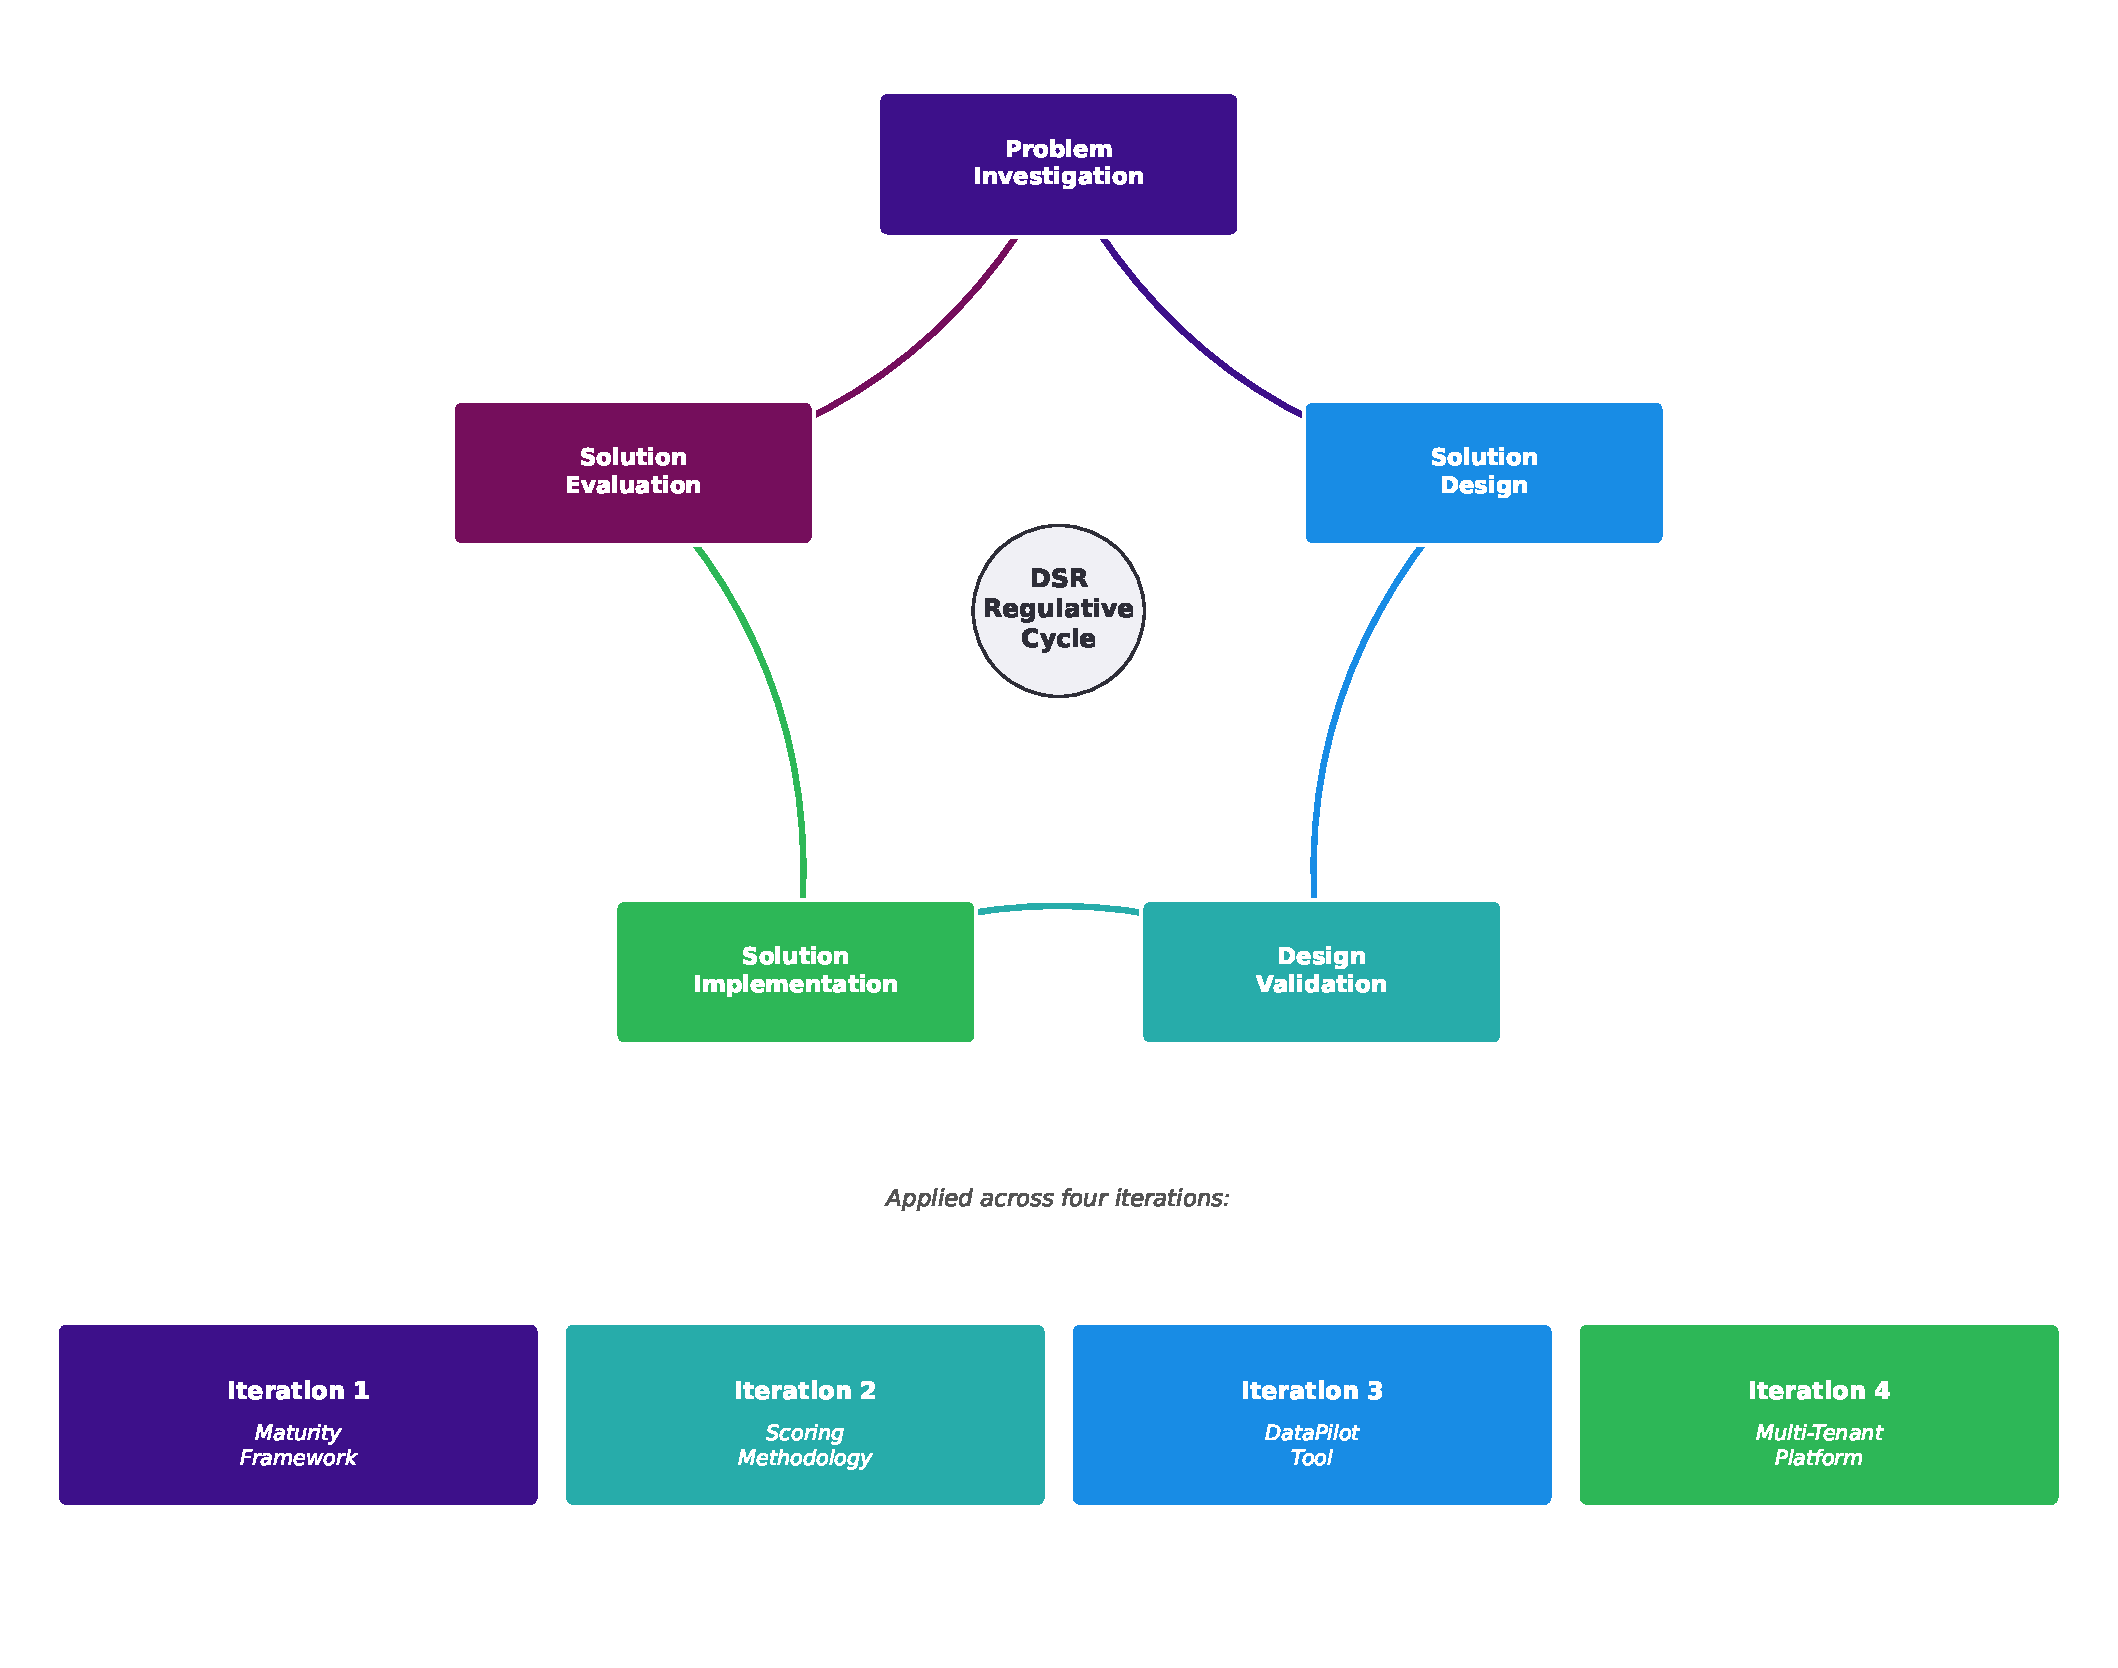
\includegraphics[width=0.85\textwidth]{images/dsr-cycle.pdf}
\caption{The DSR regulative cycle applied across the four iterations}
\label{fig:dsr-cycle}
\end{figure}

\subsection{Agile Development Approach}

The development of DataPilot requires iterative design, continuous testing, and progressive refinement, which makes an Agile approach appropriate. Scrum, one of the most widely used Agile frameworks, organizes development work through short cycles that allow the product to be improved continuously \cite{schwaber2020}. Its use is justified because the tool must be developed progressively, the scoring model and questionnaire are expected to require adjustment during development, and iterative testing improves both the usability and the accuracy of the results. Within the project, Agile principles structure the development of the tool through repeated cycles of planning, development, testing, and refinement, which complement the DSR cycle at the level of the software artifact.

\subsubsection{Combining DSR and Agile}

Design Science Research and Agile operate at two different levels and are combined deliberately rather than merged. DSR governs the research level, providing the rationale for the artifacts, the validation against requirements, and the evaluation against evidence, so that each design decision can be justified and traced. Agile governs the construction level, providing the short, feedback driven cadence through which the scoring engine and the six screens are built and refined. The two are compatible because the DSR design cycle is itself iterative, and each turn of that cycle can be realized as one or more Agile increments that deliver a working, testable slice of the tool.

Concretely, the four project iterations map onto the DSR design cycle, and the development inside each iteration is organized in the Agile manner. The first iteration designs the framework, the second designs and implements the scoring engine, the third designs and implements the DataPilot tool with its six screens, and the fourth extends that tool into the multi-tenant platform with its role model, its backend, and its group assessment workflow. Within an iteration, the five DSR activities set the goals and the acceptance criteria, while the Agile cadence of planning, development, testing, and refinement produces and stabilizes the increment. The DSR solution evaluation activity and the Agile testing and refinement steps reinforce each other, since a defect or usability problem surfaced during development is both a testing outcome and evidence that feeds the next problem investigation. This division of labor keeps the research disciplined and the engineering responsive without forcing either concern to imitate the other.

\subsection{Six-Phase Project Methodology}

Beyond the research and development methodologies, the project itself was conducted as a structured consulting engagement, following a four-step iterative logic: benchmark, hybrid design, evidence-based scoring, and tool development. This logic was translated into a work breakdown of six phases, a framing phase numbered 0 followed by five delivery phases numbered 1 to 5. Phases 0 to 3 constitute the pre-coding intellectual work of the project, in which the problem is framed, the existing situation analyzed, the needs identified, and the hybrid framework designed, while phases 4 and 5 cover the build and the deployment of the DataPilot tool. Figure~\ref{fig:phases-overview} gives an overview of the six phases, and Table~\ref{tab:project-phases} details the focus and the key deliverables of each phase.

\begin{figure}[H]
\centering
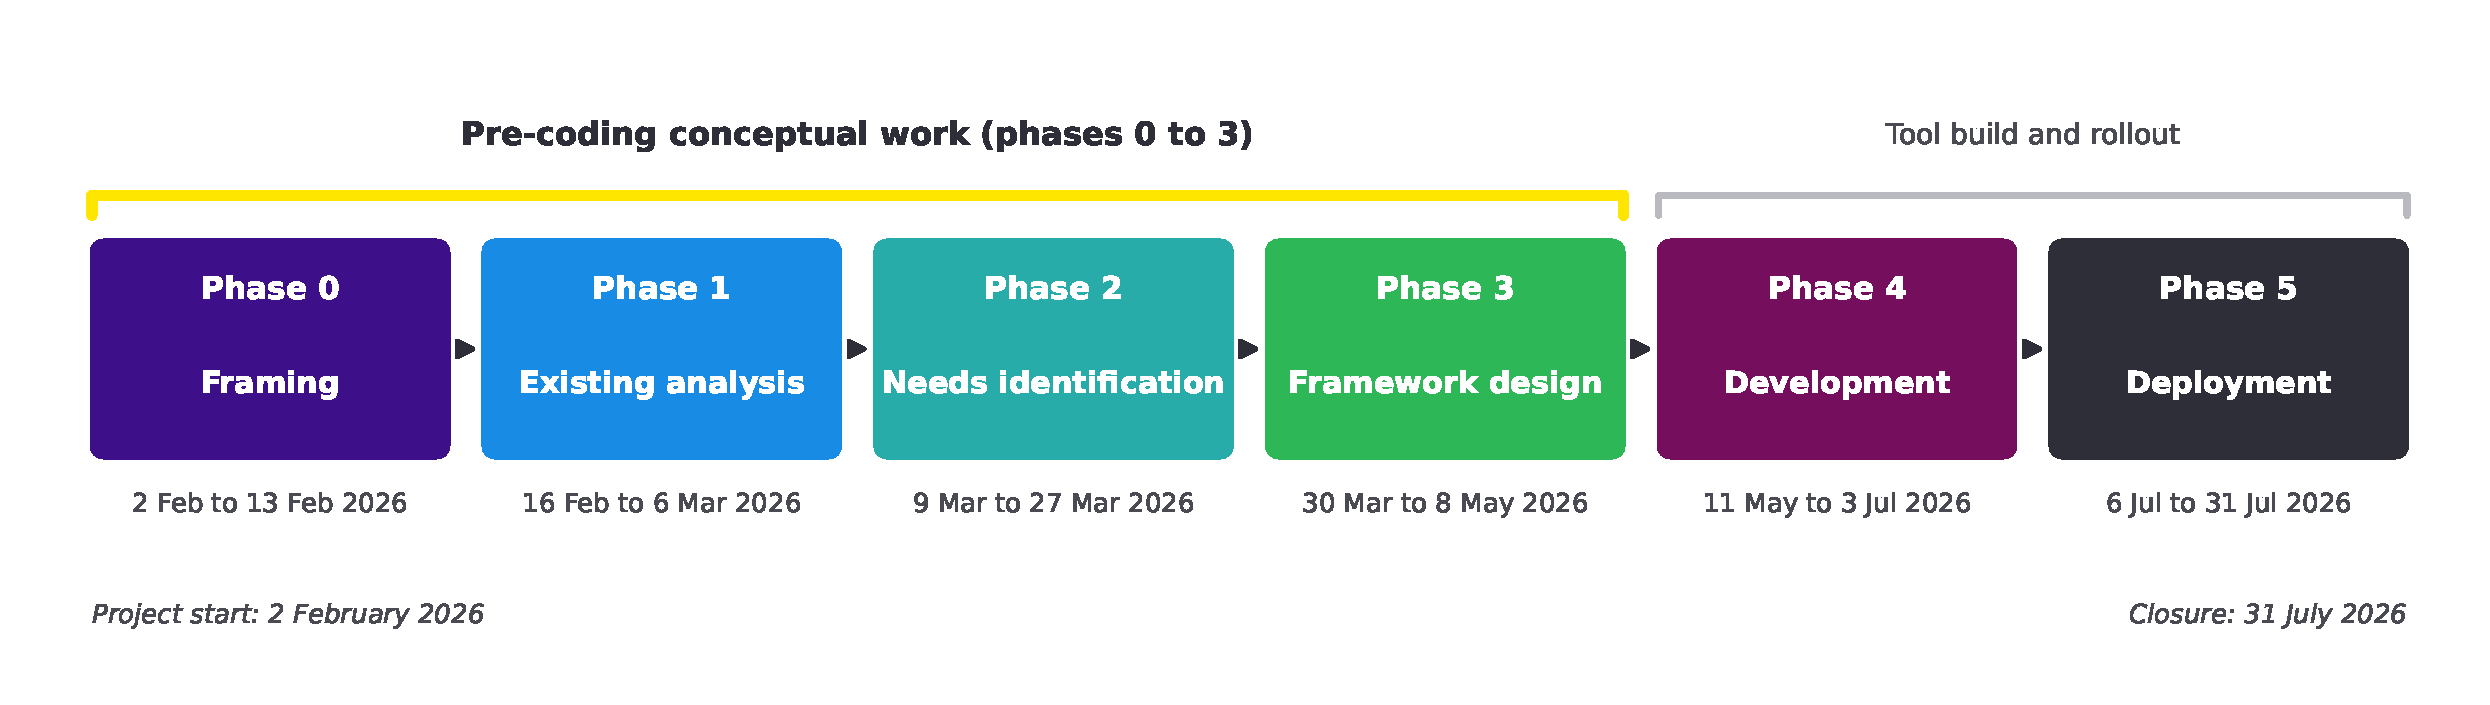
\includegraphics[width=0.95\textwidth]{images/phases-overview.pdf}
\caption{The six project phases from framing to deployment}
\label{fig:phases-overview}
\end{figure}

\begin{table}[H]
\centering
\caption{The six-phase project methodology and its key deliverables}
\label{tab:project-phases}
\footnotesize
\setlength{\tabcolsep}{4pt}
\begin{tabular}{|c|p{2.6cm}|p{5.4cm}|p{5.2cm}|}
\hline
\textbf{Phase} & \textbf{Name} & \textbf{Focus} & \textbf{Key deliverables} \\
\hline
0 & Framing (Cadrage) & Onboarding, scoping, documentary research, methodology definition, project plan, kickoff & Methodology document, project plan, kickoff presentation \\
\hline
1 & Analysis of the existing situation & Operational review, conceptual review, limits and risks, stakeholder mapping & Stakeholder map, operational and conceptual diagnostics, risks and limits report \\
\hline
2 & Needs identification & Framework study, business and data needs, functional and analytical requirements, target vision & Framework comparison synthesis, requirements specification, needs analysis report, target vision \\
\hline
3 & Framework design & Dimensions and maturity levels, scores and indicators, scoring methodology, market benchmark & Hybrid maturity framework, full scoring methodology, benchmark matrix \\
\hline
4 & Tool development & Environment setup, questionnaire, dashboards, automatic maturity calculation, functional tests & DataPilot interactive tool, functional documentation \\
\hline
5 & Deployment & Final deployment and validation, results and gap analysis, scenario and business-gain simulation, closure & Evaluation results, executive presentation, final report \\
\hline
\end{tabular}
\end{table}

The six phases and the four DSR iterations described above are two views of the same work. The first iteration, the design of the hybrid framework, is carried out through the pre-coding phases: phase 1 supplies the diagnosis of the existing situation, phase 2 the requirements and the target vision, and phase 3 the framework itself with its dimensions and maturity levels. The second iteration, the design of the scoring methodology and its engine, begins in phase 3, where the scores, indicators, and scoring methodology are constructed, and is implemented at the start of phase 4. The third iteration, the DataPilot tool with its six screens, corresponds to the build and deployment phases 4 and 5, in which the framework and the scoring engine are embodied in the interactive application, tested, and validated. The fourth iteration, the extension into the multi-tenant platform, also falls within phases 4 and 5, building on the deployed tool to add the role hierarchy, the Supabase backend, and the group assessment workflow. The phase structure thus provides the project management timeline, while the DSR iterations provide the research logic that runs through it.

That research logic can be compressed into a single view. Table~\ref{tab:dsr-iterations} summarizes the regulative cycle as it was applied in each of the four iterations, phrasing each problem investigation as the design question the iteration set out to answer, and stating for each the solution that was designed and validated, the artifact that was implemented, and the outcome of its evaluation. The table is intended as a reference point for Section 4, where each cell is developed into a full DSR activity subsection.

\begin{table}[H]
\centering
\caption{Summary of the DSR regulative cycle across the four iterations}
\label{tab:dsr-iterations}
\footnotesize
\setlength{\tabcolsep}{4pt}
\begin{tabular}{|p{0.8cm}|p{3.3cm}|p{3.7cm}|p{2.6cm}|p{3.6cm}|}
\hline
\textbf{Iter.} & \textbf{Problem investigated (design question)} & \textbf{Solution designed and validated} & \textbf{Artifact implemented} & \textbf{Evaluation outcome} \\
\hline
1 & Can the breadth of data management be structured into an assessable hierarchy aligned with the BCT Circulaire N\textdegree{}2025-08 and BCBS 239 requirements? & Hybrid structure of five dimensions, twelve sub-dimensions, and forty seven indicators; dimension weights of 25/20/20/20/15 and the mapping of the regulatory obligations onto indicators validated & Framework catalogue with a five-level rubric per indicator & Coverage of the five areas and regulatory alignment confirmed; Skills and Culture retained as a proxy-only dimension \\
\hline
2 & Can forty seven indicator scores be aggregated into a single auditable index that resists over-optimistic self-assessment? & Weighted, renormalized aggregation chain plus four business rules: the evidence requirement, the anti-gaming evidence cap, the bounded skip logic, and the non-skippable status of the thirteen regulatory indicators & Scoring engine expressed as pure store selectors & Worked example verified by hand: GMI of 2.19/5, displayed as 44\% and Level 2, Emerging; evidence cap confirmed, a score of 4 without evidence computing as 2 \\
\hline
3 & Can the framework and its scoring methodology be operationalized as an interactive tool usable by bank management? & Six-screen client-side single-page application with a completion gate protecting the result screens & The DataPilot tool & Functional testing and simulated assessment scenarios on anonymized data confirmed the fidelity of the tool to the scoring methodology \\
\hline
4 & Can one assessment be produced by many contributors across a bank, under EY oversight, without weakening confidentiality or auditability? & Four-role hierarchy with a top-down invite chain, departments with dimension-to-department assignments, per-bank copies of the EY master template, and two-layer enforcement combining row-level security with service-role endpoints & The DataPilot multi-tenant platform & Functional scenarios on the seeded demo bank confirmed the role gates, the tenant isolation, and the immutability of finalized submissions \\
\hline
\end{tabular}
\end{table}

Read row by row, the table shows the cumulative logic of the project: each iteration takes the validated output of its predecessor as its input, so the framework of the first iteration becomes the object measured by the second, and the scoring engine of the second becomes the core embedded in the third, and the tool of the third becomes the foundation that the fourth scales into a platform. Table~\ref{tab:rq-iterations} completes this view by mapping the three research questions of Section 1 onto the diagnostic survey and the four iterations, making explicit which part of the work answers which question.

\begin{table}[H]
\centering
\caption{Mapping of the research questions onto the survey and the four iterations}
\label{tab:rq-iterations}
\footnotesize
\setlength{\tabcolsep}{4pt}
\begin{tabular}{|p{1.0cm}|p{6.8cm}|c|c|c|c|c|}
\hline
\textbf{RQ} & \textbf{Focus} & \textbf{Survey} & \textbf{Iter. 1} & \textbf{Iter. 2} & \textbf{Iter. 3} & \textbf{Iter. 4} \\
\hline
RQ1 & Current state of data maturity in Tunisian banks and gaps relative to standards and regulatory requirements & X & X & & & \\
\hline
RQ2 & Design of a maturity assessment framework fitted to the Tunisian banking sector & X & X & X & & \\
\hline
RQ3 & Extent to which an interactive steering tool supports decision-making and accelerates transformation & & & X & X & X \\
\hline
\end{tabular}
\end{table}

The mapping is deliberately honest about where each answer comes from. RQ1 is answered chiefly by the diagnostic survey, with the first iteration supplying the reading grid of dimensions and indicators through which the field evidence is interpreted. RQ2 is answered by the first two iterations, which together produce the framework and the scoring methodology that make it operational, with the survey supplying the field evidence against which the design is calibrated. RQ3 is answered by the second, third, and fourth iterations, since the auditability of the score is a property of the scoring engine, its usability a property of the tool that embeds it, and its deployability across a bank and across engagements a property of the multi-tenant platform. No research question depends on a single iteration alone, which reflects the cumulative construction summarized in Table~\ref{tab:dsr-iterations}.

Across the six phases, eleven deliverables were planned, labeled L1 to L11:

\begin{itemize}
\item L1: stakeholder mapping;
\item L2: existing-situation analysis report;
\item L3: requirements specification;
\item L4: target solution description;
\item L5: data maturity framework;
\item L6: methodological documentation;
\item L7: interactive steering tool;
\item L8: functional documentation;
\item L9: evaluation results;
\item L10: executive presentation;
\item L11: final report.
\end{itemize}

Deliverables L1 to L6 belong to the pre-coding phases 0 to 3, whereas L7 to L11 are produced during the development and deployment phases 4 and 5.

\subsection{Stakeholder Analysis}

Because the framework and the tool are intended to be used inside banking institutions within an advisory engagement, a stakeholder analysis was conducted during phase 1 to identify who is affected by a data maturity assessment, what each actor expects from it, and how each actor should be engaged. Two groups of stakeholders were distinguished: the internal stakeholders of the assessed Tunisian banks, and the stakeholders of the EY mission that delivers the assessment. Table~\ref{tab:stakeholders-bank} presents the internal bank stakeholders and Table~\ref{tab:stakeholders-ey} presents the EY mission stakeholders.

\begin{table}[H]
\centering
\caption{Internal stakeholders of the Tunisian banks}
\label{tab:stakeholders-bank}
\footnotesize
\setlength{\tabcolsep}{4pt}
\begin{tabular}{|p{3.0cm}|p{4.6cm}|p{6.9cm}|}
\hline
\textbf{Stakeholder} & \textbf{Role} & \textbf{Interest} \\
\hline
Chief Data Officer & Responsible for data governance & Steer the transformation plan and track the evolution of the maturity level \\
\hline
Data Manager & Operational coordination of data management & Structure improvement initiatives and strengthen data processes \\
\hline
Data Owners & Owners of business data & Improve the quality, traceability, and reliability of data in their scope \\
\hline
Risk Manager & Supervision of data-related risks & Ensure control of operational and regulatory data risks \\
\hline
IT Manager & Management of infrastructure and information systems & Anticipate the technical and budgetary impacts of recommendations \\
\hline
Data Architect & Design of the target data architecture & Align the architecture with expected maturity standards \\
\hline
Compliance Officer & Guarantor of regulatory compliance & Verify the alignment of the data mechanism with regulatory requirements \\
\hline
Internal Audit & Independent control of the mechanism & Evaluate the effectiveness of the data governance framework and action plans \\
\hline
Governing body / Board & Strategic sponsor and budget decision-maker & Obtain a consolidated view of data maturity to orient strategy and prioritize investments \\
\hline
\end{tabular}
\end{table}

\begin{table}[H]
\centering
\caption{Stakeholders of the EY mission}
\label{tab:stakeholders-ey}
\footnotesize
\setlength{\tabcolsep}{4pt}
\begin{tabular}{|p{3.0cm}|p{4.6cm}|p{6.9cm}|}
\hline
\textbf{Stakeholder} & \textbf{Role} & \textbf{Interest} \\
\hline
EY Partner & Global responsibility for the mission & Commercial performance and reputation \\
\hline
Engagement Manager & Operational steering of the mission & Respect of deadlines, quality, deliverables \\
\hline
Project team (consultants) & Interviews, scoring, and analysis & Sound methodological execution \\
\hline
Sector experts & Banking expertise input & Guarantee regulatory relevance \\
\hline
\end{tabular}
\end{table}

The stakeholders were then positioned on an interest and influence matrix to plan their engagement. The actors combining high interest and high influence, namely the Chief Data Officer, the governing body or board, the EY Partner, the Engagement Manager, and the project team, are those who must be managed most closely, since they both drive the assessment and act on its results. The remaining actors, the IT Manager, Internal Audit, the sector experts, the Risk Manager, the Compliance Officer, the Data Manager, the Data Owners, and the Data Architect, were positioned according to their respective interest and influence, which determines whether they are to be kept satisfied, kept informed, or simply monitored during the engagement. Figure~\ref{fig:stakeholder-matrix} presents the matrix. The resulting stakeholder cartography constitutes deliverable L1 and was presented in the weekly meeting of 24 February 2026.

\begin{figure}[H]
\centering
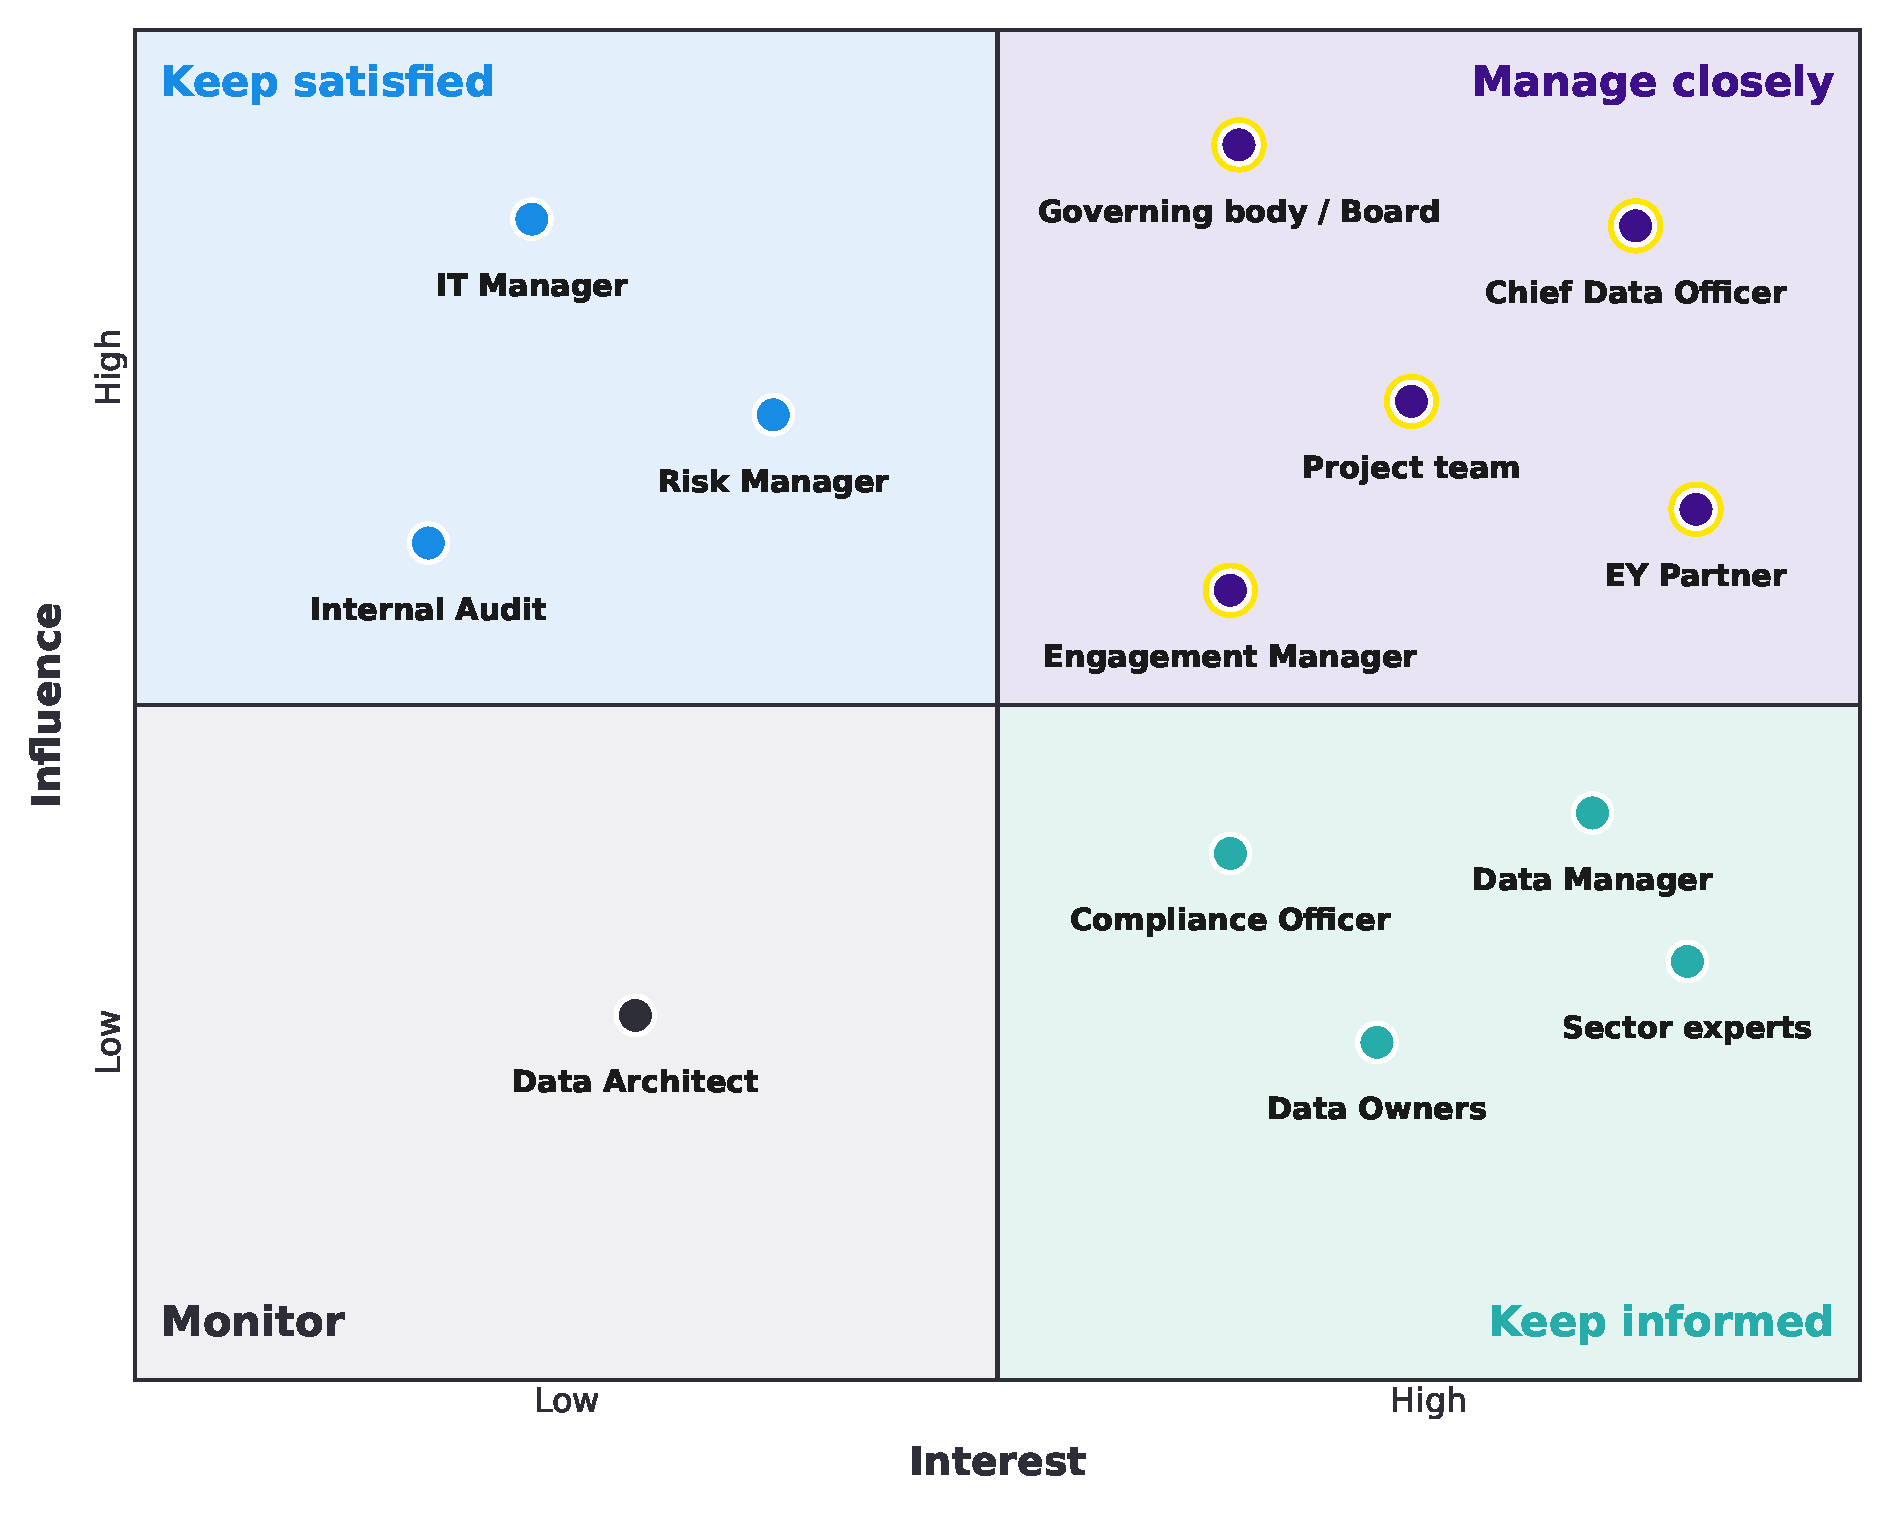
\includegraphics[width=0.8\textwidth]{images/stakeholder-matrix.pdf}
\caption{Stakeholder interest and influence matrix}
\label{fig:stakeholder-matrix}
\end{figure}

\subsection{Planning and Work Breakdown}

The project was conducted at EY Tunisia over a 24-week plan. It started on 2 February 2026 with the framing phase, and the kickoff presentation was delivered on 12 February 2026. The pre-coding phases 0 to 3 run from 2 February to early May 2026 and carry the intellectual work described above, from framing through the design of the hybrid framework and its scoring methodology. Development of the DataPilot tool begins on 11 May 2026, and the project closes with the deployment phase ending on 31 July 2026. In addition to the six phases, a transversal workstream covers report writing, risk management, and project steering with weekly meetings throughout the engagement. Table~\ref{tab:phase-timeline} presents the phase-level timeline with the key tasks of each phase, and the resulting schedule is visualized as a Gantt chart in Figure~\ref{fig:gantt}. Of the planned tasks, the scenario and business-gain simulation was realized in the delivered tool as target-level setting and gap-to-target visualization, with the quantitative what-if simulation of business gains identified as future work, as stated in Sections 5 and 7.

\begin{table}[H]
\centering
\caption{Phase-level timeline and work breakdown of the 24-week plan}
\label{tab:phase-timeline}
\footnotesize
\setlength{\tabcolsep}{4pt}
\begin{tabular}{|p{3.2cm}|p{3.2cm}|p{8.4cm}|}
\hline
\textbf{Phase} & \textbf{Period} & \textbf{Key tasks} \\
\hline
Phase 0: Framing & 2 February to 13 February 2026 & Team integration; project scoping; benchmark and documentary research; methodology definition; project plan; kickoff preparation and presentation \\
\hline
Phase 1: Existing analysis & 16 February to 6 March 2026 & Stakeholder cartography; operational review; conceptual review; identification of limits and risks \\
\hline
Phase 2: Needs identification & 9 March to 27 March 2026 & Study of existing maturity frameworks; business and data needs analysis; functional and analytical requirements; target vision definition \\
\hline
Phase 3: Framework design & 30 March to 8 May 2026 & Dimensions and maturity levels; scores and indicators; scoring methodology construction; benchmark against market best practice \\
\hline
Phase 4: Development & 11 May to 3 July 2026 & Development environment setup; questionnaire implementation; dashboard design; automatic maturity calculation; functional and non-regression tests; scenario and business-gain simulation \\
\hline
Phase 5: Deployment & 6 July to 31 July 2026 & Final deployment and validation; results and maturity-gap analysis; final restitution and project closure \\
\hline
Transversal & 16 February to 31 July 2026 & Report writing; risk management; project steering and weekly meetings \\
\hline
\end{tabular}
\end{table}

\begin{figure}[H]
\centering
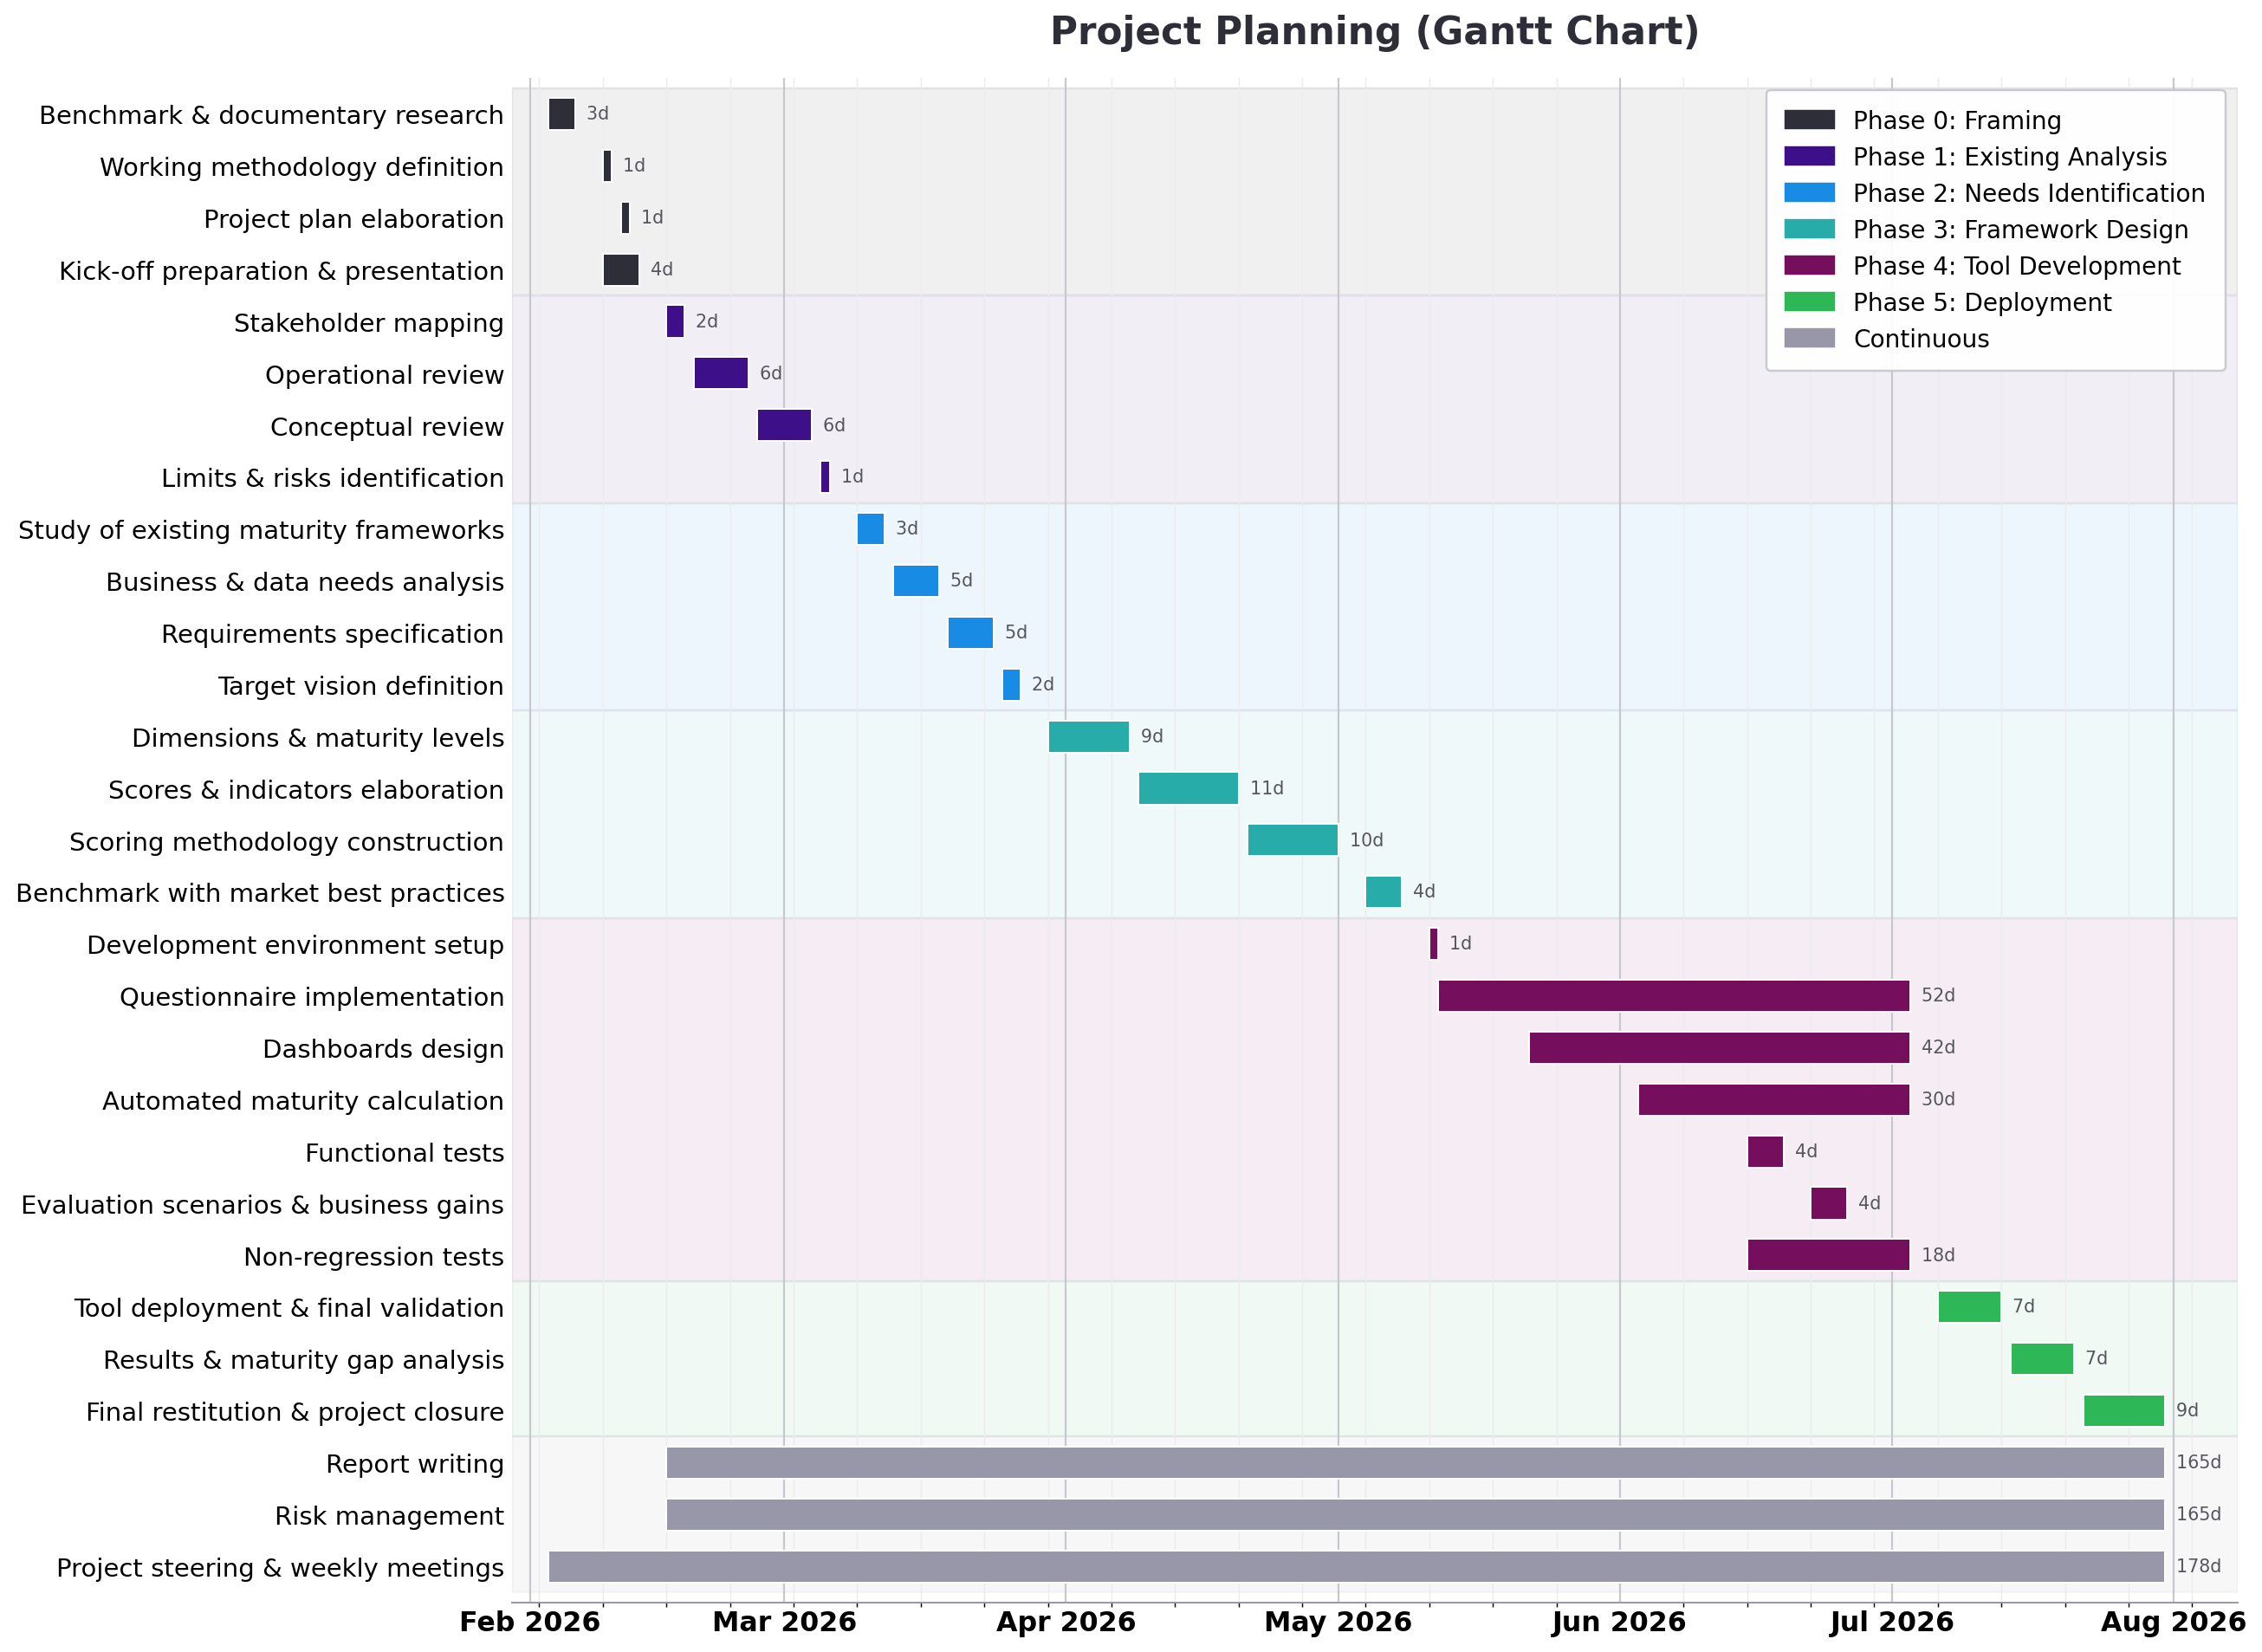
\includegraphics[width=\textwidth]{images/gantt-planning.png}
\caption{Project planning (Gantt chart)}
\label{fig:gantt}
\end{figure}

\subsection{Research Materials}

The design of the framework is grounded in two categories of research materials. The first is a diagnostic survey of 44 banking professionals, which provides the field evidence on the current state of data governance, quality, architecture, analytics, and culture in the sector, and which informs both the diagnosis and the calibration of the framework. The second is a benchmark that screened fifteen international data maturity frameworks and retained five, DAMA-DMBOK, DCAM, CMMI-DMM, TDWI, and Gartner, whose comparative analysis, presented in Section 2, determines the role retained from each in the hybrid model. Together, these materials ensure that the framework is grounded both in the field reality of the sector and in the established state of practice.

\subsubsection{Diagnostic Survey Design}

The diagnostic survey is the principal source of field evidence for the relevance cycle. It was administered to 44 professionals working in the Tunisian banking sector, in roles connected to data, such as data management, information technology, risk, compliance, and analytics functions, so that the responses reflect the perspective of practitioners who deal with the sector data challenges directly. The survey serves two purposes at once. It establishes the diagnosis of the current state of the sector across the areas that the framework covers, and it informs the calibration of the framework by revealing which questions discriminate between organizations and where practices are weakest.

The instrument is organized around the same five areas that structure the framework: governance, data quality, architecture and access, analytics and tools, and skills and culture. Aligning the survey with the five dimensions ensures that the field evidence maps cleanly onto the framework being designed, so that a weakness observed in a given area in the survey can be traced to the corresponding dimension, sub-dimension, and indicators. The questions were expressed in terms accessible to practitioners and phrased so that answers describe observable practices rather than opinions, which supports the later principle, embodied in the tool, that a claimed level of maturity must be backed by evidence.

Several limitations of the survey are acknowledged and shape how its results are used. The sample of 44 respondents is modest and was gathered by reaching professionals who were accessible during the project, so it is not a strict probability sample of the sector and the findings are indicative rather than statistically representative. Responses are self reported, which introduces the risk that respondents present their organization more favorably than the underlying practices warrant, a risk that the framework mitigates through the evidence cap applied in the scoring engine. The skills and culture dimension is particularly difficult to observe directly, which is why it is assessed through proxy indicators only. For these reasons the survey is treated as a diagnostic and calibration input, not as a validation of the framework, and the numeric results reported in Section 5 are interpreted with these constraints in mind.

\subsection{Research Ethics and Data Handling}

Because the diagnostic survey involves human participants and the tool records evidence describing internal banking practices, the project applies a set of ethical and data handling principles consistent with the confidentiality expectations of the sector and of the host organization. Participation in the survey was voluntary, and responses were used solely for the purposes of the diagnosis and the calibration of the framework. Results are reported in aggregate across the sector rather than attributed to any named institution or individual, so that no single bank or respondent can be identified from the figures presented in Section 5.

The design of the tool reinforces this posture, and the mechanism evolved with the tool. In the single-user build of the third iteration, DataPilot ran entirely in the browser and persisted all assessment data only in the local storage of the user browser, so that nothing left the assessing institution's machine. In the delivered platform, in-progress solo answers still remain in the assessor's browser under the key \texttt{datapilot-assessment}, but submitted results, group assessments, user profiles, and per-bank questionnaire copies are stored in the platform's Postgres database, where row-level security confines every row to its own bank, with EY oversight excepted by design. Access to the platform is invite-only with no public sign-up, submissions are immutable once recorded, and the evidence fields are still intended to reference internal documents rather than to reproduce them, which limits the exposure of confidential material within the tool. The confidentiality argument thus rests on tenant isolation enforced in the database rather than on local custody alone, and these measures align the research with the confidentiality obligations of a banking engagement and reduce the risk associated with handling sensitive organizational information.

\subsection{Technologies and Tools}

\subsubsection{Tools}

The framework and its documentation were produced with standard office and modeling tools, and the diagnostic survey was collected and analyzed with a spreadsheet based workflow. The project planning was managed through a Gantt based schedule. The development of the tool was managed with Git for version control, with the codebase hosted on GitHub in the \texttt{ZizouX0/datapilot\_EY} repository, where changes were developed on dedicated branches and integrated through pull requests. Dependencies were managed with the npm package manager, code quality was enforced with ESLint configured with the React Hooks and React Refresh plugins, and the application was built and served during development with the Vite toolchain.

\subsubsection{Technologies}

The DataPilot tool is implemented as a single-page web application. The front end is built with React 19 and the Vite 8 build tool. Navigation between the screens is handled with React Router 7, using route based code splitting so that each screen and its chart dependencies are loaded on demand, which keeps the initial load light and isolates the heavier visualization code to the screens that need it. The application state is managed with Zustand 5, organized as eight stores that hold the session, the questionnaire content, and the assessment state; a solo assessment in progress is persisted to the browser local storage so that it survives page reloads. The user interface is styled with Tailwind CSS 4, the data visualizations are produced with Recharts 3, and the report export is handled with react-to-print 3, which produces a printable version of the dashboards. The fourth iteration extends this front end stack, otherwise unchanged, with a backend: Supabase provides the Postgres database that holds all tenant data under row-level security, the invite based authentication, and the file storage, reached from the browser through the Supabase JavaScript client 2 under the public key, while a small set of serverless functions carries the privileged operations that must not be possible from the browser. The application chrome is fully bilingual, English and French, through a hand-rolled internationalization layer, and the language preference follows the user across devices. Table~\ref{tab:tech-stack} summarizes this stack, associating each component of the application with the technology that implements it and the role it plays in the tool.

\begin{table}[H]
\centering
\caption{Technology stack of the DataPilot tool}
\label{tab:tech-stack}
\footnotesize
\setlength{\tabcolsep}{4pt}
\begin{tabular}{|p{3.4cm}|p{3.2cm}|p{7.6cm}|}
\hline
\textbf{Component} & \textbf{Technology} & \textbf{Role in DataPilot} \\
\hline
User interface framework & React 19 & Component based construction of the application screens \\
\hline
Build tool & Vite 8 & Development server and production build of the application \\
\hline
Navigation & React Router 7 & Routing between the screens with route based code splitting \\
\hline
State management & Zustand 5 & Central stores (eight) holding session, questionnaire content, and assessment state; the solo assessment persists to browser local storage under the key \texttt{datapilot-assessment} \\
\hline
Styling & Tailwind CSS 4 & Utility based styling of the user interface \\
\hline
Data visualization & Recharts 3 & Radar chart and dimension bar charts of the dashboards \\
\hline
Report export & react-to-print 3 & Printable version of the dashboards \\
\hline
Backend platform & Supabase & Postgres database with row-level security for tenant data, authentication with invite emails, and file storage \\
\hline
Backend access & Supabase JS client 2 & Database and authentication calls from the browser under the public key and row-level security \\
\hline
Privileged operations & Serverless functions (\texttt{api/}) & Invitations, role and account management, and the optional AI roadmap endpoint, holding the server-only service key \\
\hline
Internationalization & Hand-rolled EN/FR dictionary & Bilingual English and French application and report chrome; the language preference follows the user across devices \\
\hline
\end{tabular}
\end{table}

These technologies were selected for their suitability to a responsive, interactive, and maintainable assessment application. The client-side single-page architecture was chosen in the third iteration because, at that stage of the project, it kept the assessment data local to the user machine and avoided the need for a back end server or a hosted database; the architecture is retained in the platform because React with a lightweight state store such as Zustand keeps the scoring logic, the aggregation chain, the evidence cap, the skip logic, and the renormalization, expressed as pure selectors that can be reasoned about and tested independently of the user interface. Extracted into a pure function module, the scoring engine is shared unchanged by the solo and the group assessment paths, so both compute their scores identically and remain faithful to the methodology of the second iteration. The fourth iteration then adds a deliberately thin backend, introduced for multi-tenant isolation: the database itself enforces tenant isolation and role scope through row-level security policies, so that every row is confined to its own bank at the data layer, while the small set of serverless endpoints performs only the operations that must not be possible from the browser, namely invitations, role changes, account and department management, self-service profile updates, and the optional roadmap generation, and the role-gated endpoints among them re-check the caller's role against the database on every request. Client-side route guards remain, but as user experience only; enforcement lives in the database policies and the privileged endpoints. This division preserves the separation between the scoring logic and the presentation, which is what allows the same engine to feed the results, the gap analysis, the compliance screens, and the group assessment finalization consistently, and it directly supports the fidelity of the tool to the underlying framework.

\subsection{Conclusion}

This section presented the combined methodological approach of the project, Design Science Research for the design and validation of the artifacts and Agile principles for the development of the tool, together with the research materials and the technologies used. The next section presents the iterations through which the artifacts were produced.
